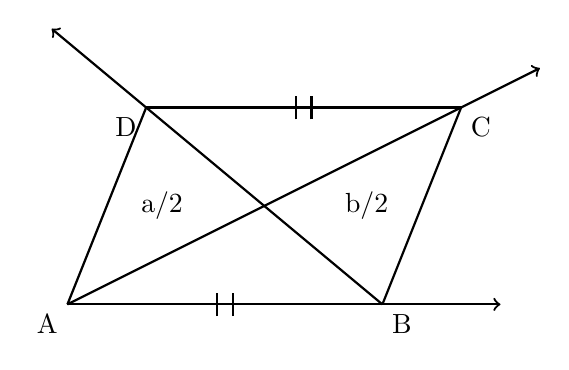
\begin{tikzpicture}[scale=1]

  % Define the vertices of the parallelogram
  \coordinate (A) at (0, 0);
  \coordinate (B) at (4, 0);
  \coordinate (C) at (5, 2.5);
  \coordinate (D) at (1, 2.5);

  % Draw the solid segments of the parallelogram that do not have arrows
  \draw[thick] (A) -- (D);
  \draw[thick] (D) -- (C);
  \draw[thick] (B) -- (C);

  % Draw the ray starting from A, passing through B, with an arrow at the end
  \draw[thick, ->] (A) -- (5.5, 0);

  % Draw the ray starting from A, passing through C, with an arrow at the end
  % The line follows the slope of AC. Extending it to x=6 gives y=3.
  \draw[thick, ->] (A) -- (6, 3);

  % Draw the ray starting from B, passing through D, with an arrow at the end
  % The line follows the slope of BD. Extending it to x=-0.2 gives y=3.5.
  \draw[thick, ->] (B) -- (-0.2, 3.5);

  % Add double tick marks on segment AB to indicate equal length
  % Centered around the midpoint (2, 0)
  \draw[thick] (1.9, -0.15) -- (1.9, 0.15);
  \draw[thick] (2.1, -0.15) -- (2.1, 0.15);

  % Add double tick marks on segment DC to indicate equal length
  % Centered around the midpoint (3, 2.5)
  \draw[thick] (2.9, 2.35) -- (2.9, 2.65);
  \draw[thick] (3.1, 2.35) -- (3.1, 2.65);

  % Add labels for the vertices exactly where they appear
  \node[below left] at (A) {A};
  \node[below right] at (B) {B};
  \node[below right] at (C) {C};
  \node[below left] at (D) {D};

  % Add measurement/region labels (a/2 and b/2) inside the respective triangles
  \node at (1.2, 1.25) {a/2};
  \node at (3.8, 1.25) {b/2};

\end{tikzpicture}